\chapter{Obecné seznámení s formáty XML a JSON}
V této kapitole seznámím čtenáře se značkovacím jazykem XML a následně s JSONem, formátem pro výměnu dat. Mým cílem je popsat základní charakteristiky a syntaxi obou formátů tak, abych byl já, a následně i čtenář, schopen pochopit v kapitole \ref{kapitolaSpecifickeAlgoritmy} principy a výhody vybraných algoritmů využívajících znalosti struktury datových souborů.

\section{XML}
Na základě značkovacího jazyka SGML (Standard Generalized Markup Language), jehož obecnost činí úplnou implementaci velmi náročnou, vznikl vybráním nejpoužívanějších možností nový značkovací jazyk XML (eXtensible Markup Language), je tedy podmnožinou jazyka SGML. XML je obecný a otevřený, jeho vývoj a standardizaci realizovalo konsorcium W3C (World Wide Web Consorcium) \cite{w3cxml}. XML umožňuje snadné vytváření konkrétních značkovacích jazyků pro popis dokumentů a dat ve standardizované, textově orientované podobě. 

\subsection{Charakteristika}


\subsection{Syntaktická analýza}
V podstatě jde o textový dokument, je tvořen posloupností Unicode\footnote{Unicode je standard pro konzistentní kódování, reprezentaci a manipulaci znaků většiny světových abeced.} znaků, ve kterém se rozlišují dva základní prvky: elementy neboli značky a obsah. Při práci s XML je nutné mít na paměti, že je na dodržení syntaxe kladen velmi velký důraz. Při dodržení správného způsobu zápisu a pravidel, která budou popsána níže, lze dokument považovat za tzv. \textit{well-formed XML} \cite{w3cxml}.

\subsubsection{Element}
Základním prvkem každého XML dokumentu je element, který je vyznačen pomocí takzvaných tagů\footnote{Tag definuje formu části textu.}, mezi které může být vložen obsah. Počáteční i ukončující tag je dle definice \cite{w3cxml} složen z dvojice znamének \texttt{<} (menší než) a \texttt{>} (větší než), mezi kterými je zapsán název tagu a volitelně i atributy. Ukončovací tag má navíc před svým názvem znak \texttt{/} (lomeno). Při správné aplikaci pravidel může vypadat element například následujícím způsobem:
$$\texttt{<název\_elementu název\_atributu=\textquotedblright hodnota atributu\textquotedblright></název\_elementu>}.$$
V případě, že element neobsahuje žádný obsah, lze ho zkráceně zapsat jako tzv. prázdný element:
$$\texttt{<název\_prázdného\_elementu />}.$$
V případě nedodržení správné syntaxe může nastat problém při rozpoznávání zapsaných dat, což může mít za následek nekompatibilitu mezi různými systémy při výměně dat.

\subsubsection{Atribut}
Počáteční tag elementu může obsahovat atributy upřesňující jeho význam. Atribut je vždy složen ze svého názvu a hodnoty, které jsou odděleny znakem \texttt{=} (rovná se). Hodnota je navíc zapsána mezi dvojici znaků \texttt{\textquotedblright} (uvozovky) nebo \texttt{\textquoteright} (apostrof), přičemž hodnota může obsahovat jeden z těchto znaků tak, že se syntakticky nekříží. Následuje příklad atributu, jehož hodnota obsahuje znak \texttt{\textquoteright}:
$$\texttt{název\_atributu=\textquotedblright hodnota atributu osahující znak \textquoteright\ (apostrof)\textquotedblright}.$$

\subsubsection{Obsah}
Vše, co není tagem, je v dokumentu považováno za obsah. Kromě obyčejného textu mohou být obsahem další vnořené elementy, komentáře, instrukce pro zpracování, reference a další. Vzhledem k tomu, že určité znaky mají v syntaxi XML speciální význam (např. \texttt{<}, \texttt{>}), využívají se pro jejich zápis znakové entity\footnote{Pomocí znakových entit (sekvence znaků) lze zapsat znaky, které neobsahuje zvolená znaková sada, nebo mají v použitém kontextu speciální význam.}. Úplný výčet toho, co může XML dokument obsahovat, je včetně pravidel definován v \cite{w3cxml}.

\subsection{Vzorový příklad}
\label{xmlpriklad}
Na následujících řádcích je zapsán XML element typu \texttt{Person}, oblíbená postavička Homer Simpson ze seriálu The Simpsons, který kromě jiného obsahuje vnořený element typu \texttt{Relatives}, který zde slouží jako kontejner s Homerovými příbuznými.

\texttt{\small<Person>\\
\hspace*{2mm}<FirstName>Homer</FirstName>\\
\hspace*{2mm}<LastName>Simpson</LastName>\\
\hspace*{2mm}<Relatives>\\
\hspace*{4mm}<Relative>Grandpa</Relative>\\
\hspace*{4mm}<Relative>Marge</Relative>\\
\hspace*{4mm}<Relative>Bart</Relative>\\
\hspace*{4mm}<Relative>Lisa</Relative>\\
\hspace*{4mm}<Relative>Maggie</Relative>\\
\hspace*{2mm}</Relatives>\\
</Person>}


\subsection{Parsování}


\section{JSON}
JSON neboli JavaScript Object Notation je odlehčený způsob zápisu (formátování) dat. Tento textový formát je nezávislý na počítačové platformě a je čitelný pro člověka. JSON je založen na dvou univerzálních datových strukturách: kolekce dvojic klíč/hodnota s unikátními klíči (tzv. associative array) a seřazený seznam hodnot (tzv. array), které podporují v nějaké formě asi všechny známé moderní programovací jazyky. Díky těmto vlastnostem se JSON stal velmi oblíbeným formátem pro vzájemnou výměnu dat.

\subsection{Charakteristika}


\subsection{Syntaktická analýza}
Jak již bylo zmíněno, je JSON textový formát a je tedy posloupností tokenů tvořených z Unicode znaků. Sada tokenů obsahuje šest strukturálních tokenů: \texttt{[} (levá hranatá závorka), \texttt{\{} (levá složená závorka), \texttt{]} (pravá hranatá závorka), \texttt{\}} (pravá složená závorka), \texttt{:} (dvojtečka) a \texttt{,} (čárka); dále obsahuje znakové řetězce, čísla a tři doslovné tokeny: \texttt{true}, \texttt{false} a \texttt{null}.

\subsubsection{Hodnoty}
Za hodnotu je v JSONu považován objekt, pole, číslo, řetězec, \texttt{true}, \texttt{false}, nebo \texttt{null}.

\begin{figure}[!htb]
\centering
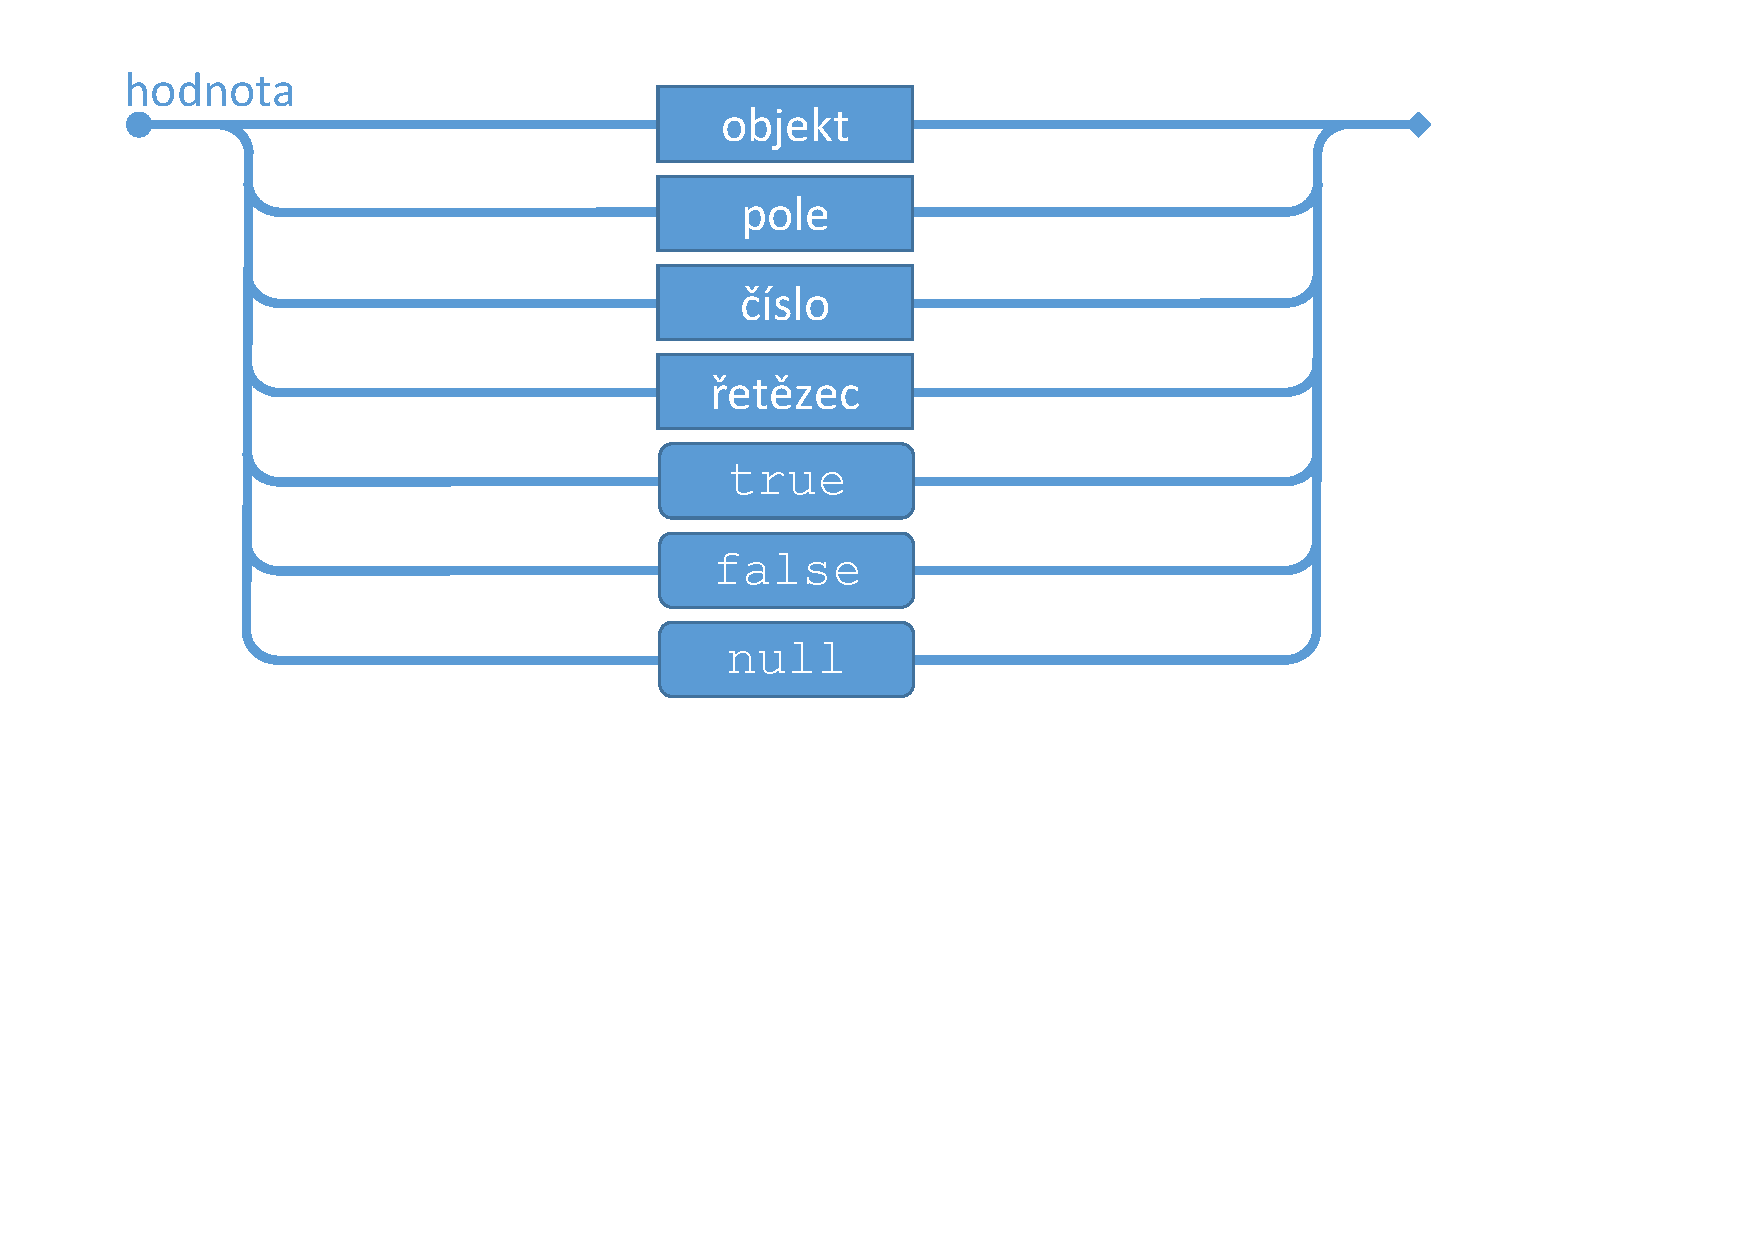
\includegraphics[trim=0 260 90 30, clip, angle=0, width=150mm]{hodnota}
\caption{Struktura hodnoty}
\label{hodnota}
\end{figure}

\subsubsection{Objekty}
Objekt je reprezentován dvojicí složených závorek, uvnitř kterých je žádná nebo více dvojic klíč/hodnota, přičemž klíč je řetězec. Klíč a hodnota jsou odděleny dvojtečkou a jednotlivé dvojice odděluje čárka.

\begin{figure}[!htb]
\centering
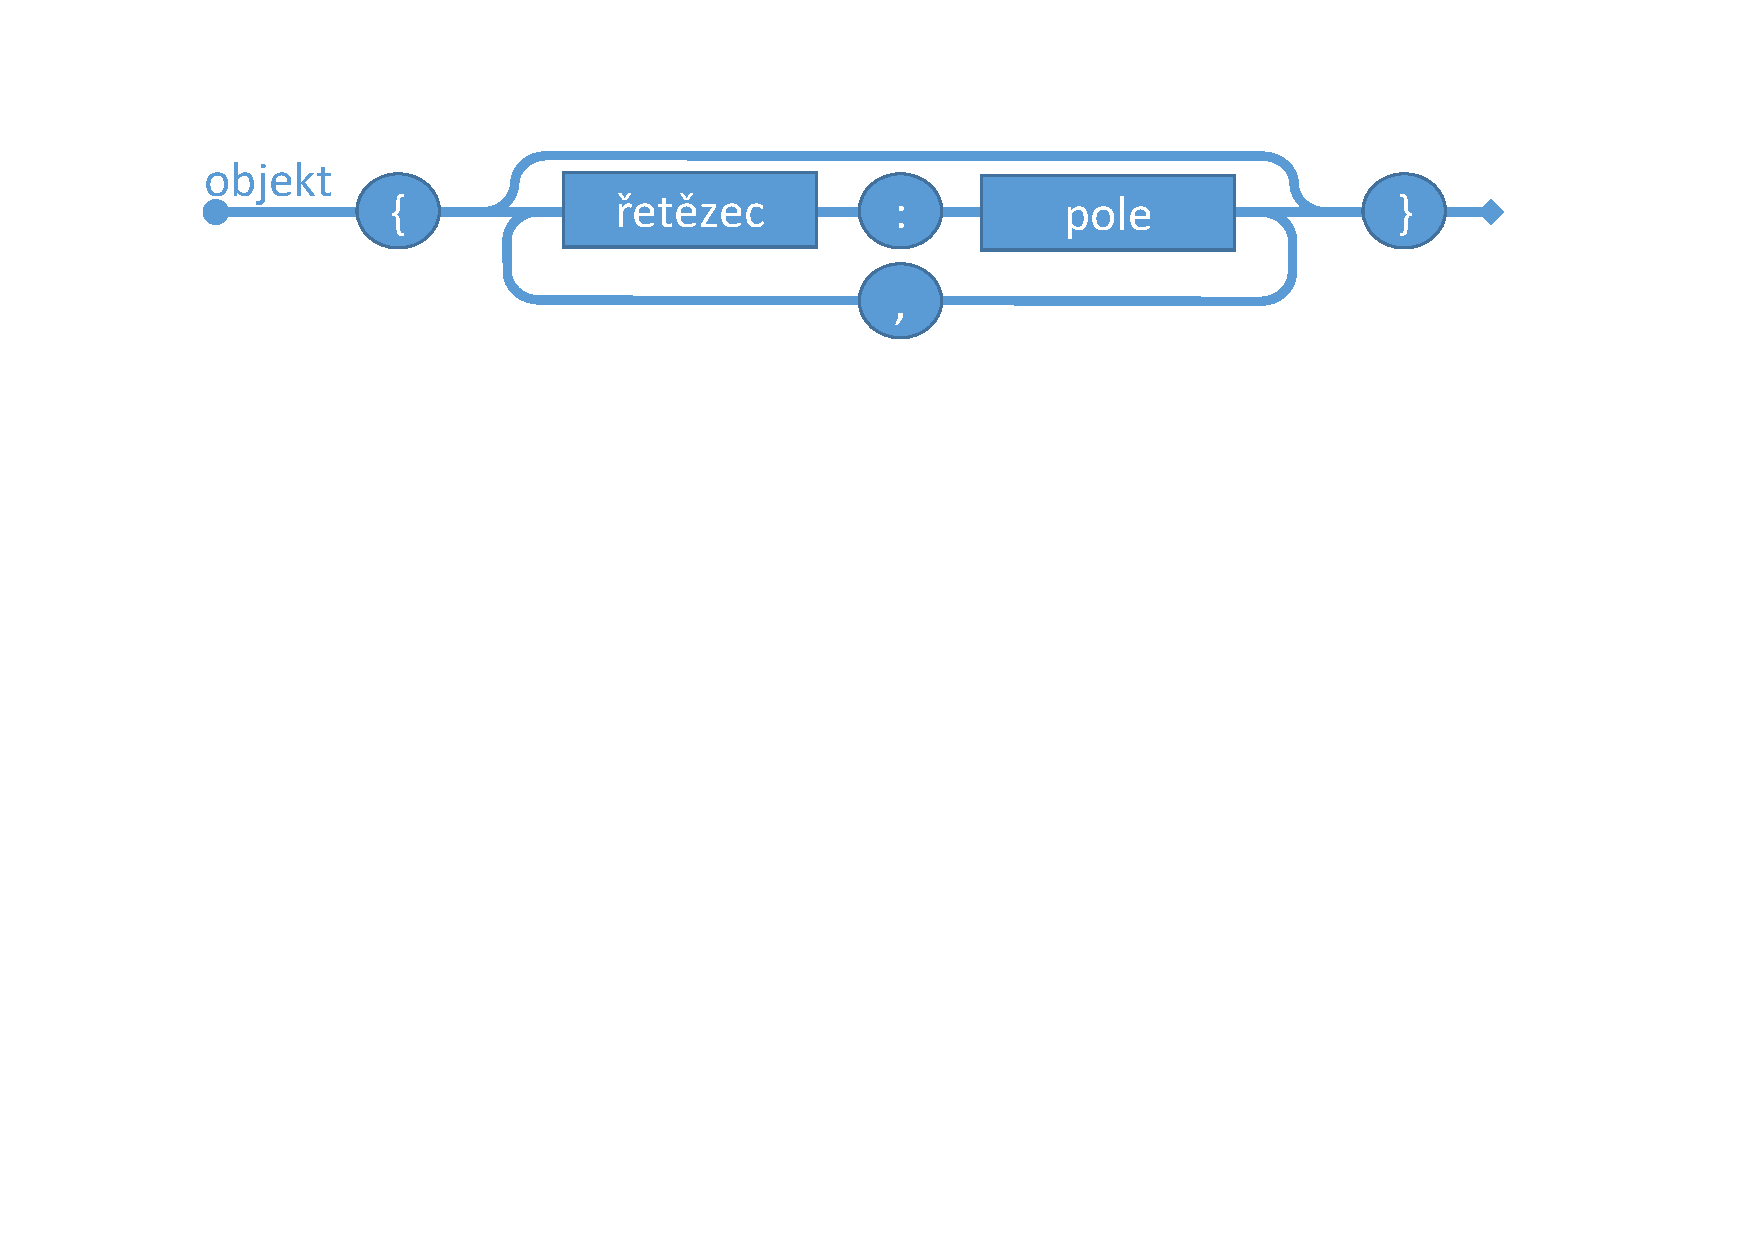
\includegraphics[trim=70 430 80 70, clip, angle=0, width=150mm]{objekt}
\caption{Struktura objektu}
\label{objekt}
\end{figure}

\subsubsection{Pole}
Pole je složeno z dvojice hranatých závorek, mezi kterými může být nula nebo více seřazených hodnot, které jsou odděleny čárkou.

\begin{figure}[!htb]
\centering
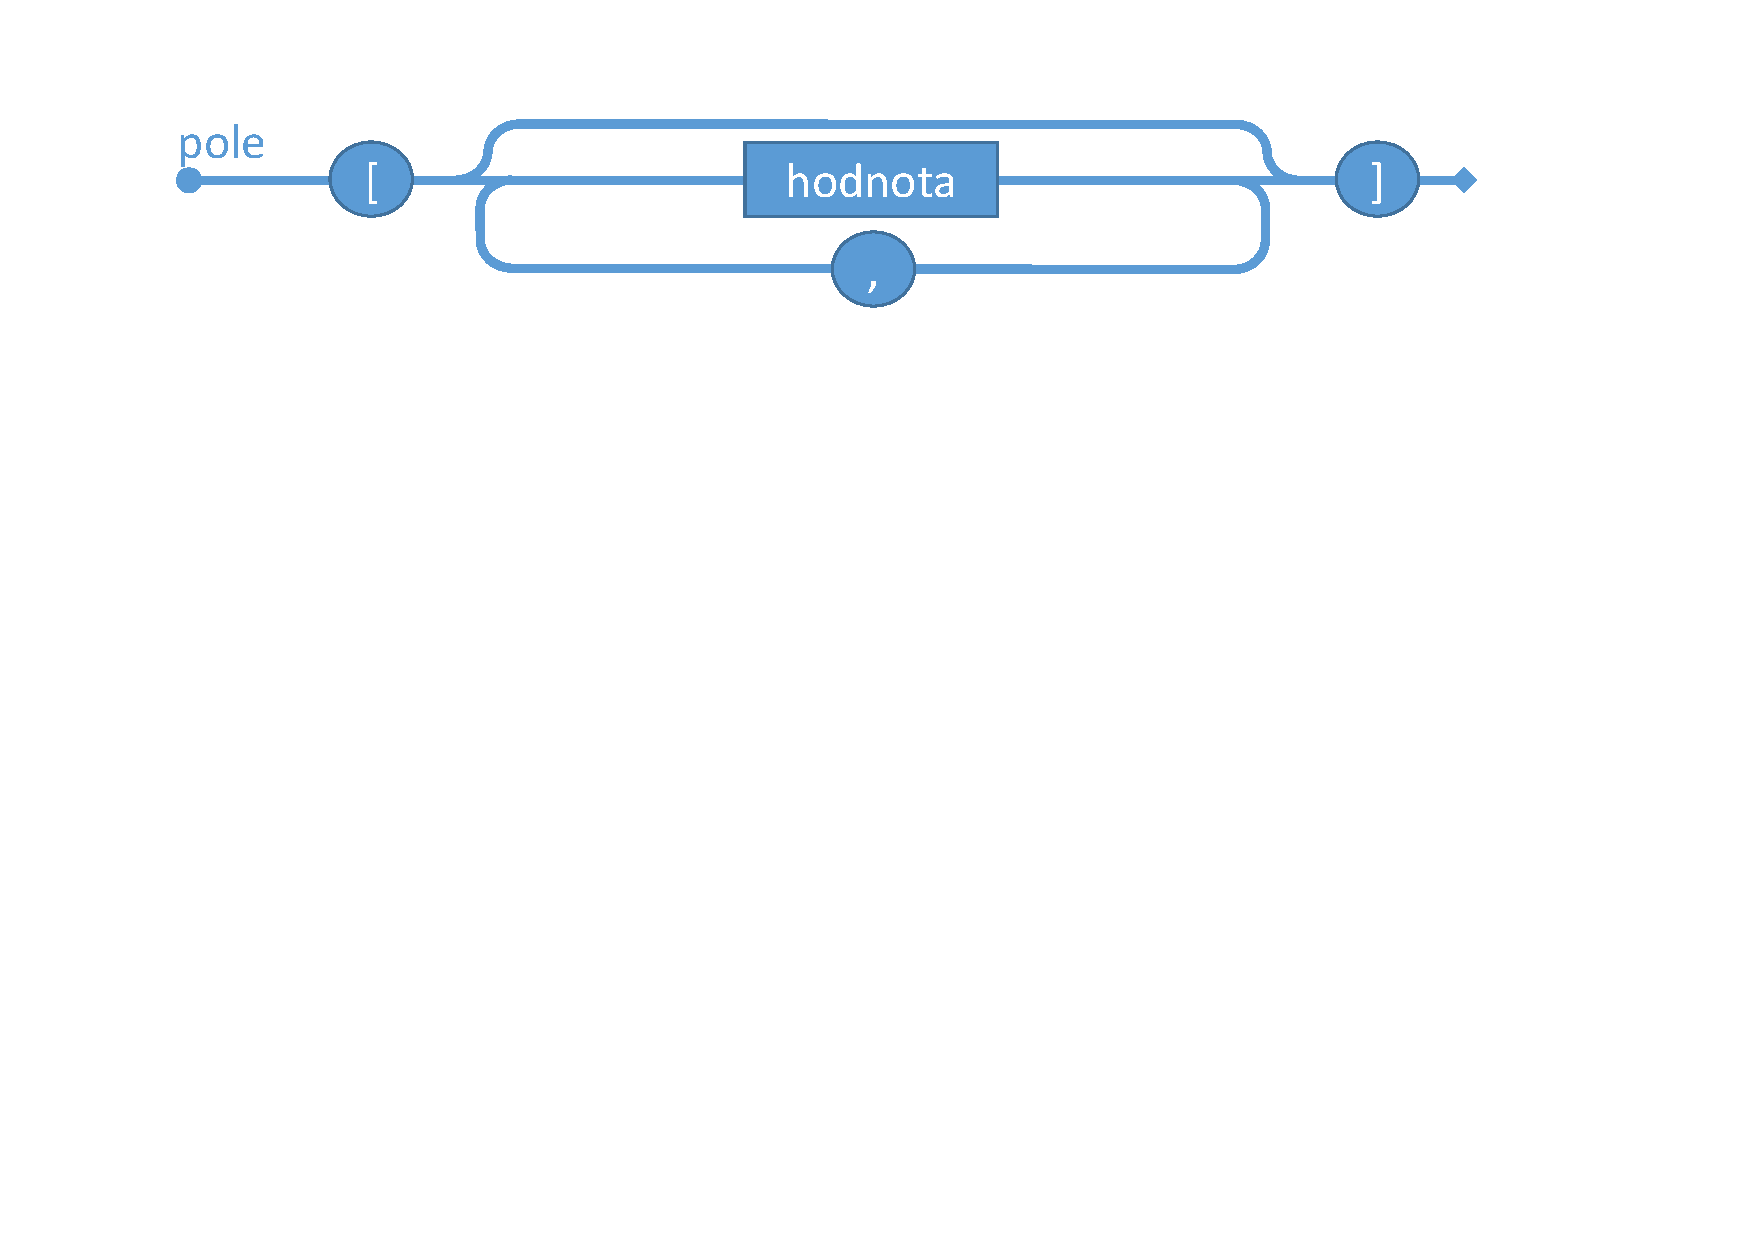
\includegraphics[trim=60 445 90 55, clip, angle=0, width=150mm]{pole}
\caption{Struktura pole}
\label{pole}
\end{figure}

\subsubsection{Čísla}
Čísla jsou v desítkové soustavě (tedy číslice $0 - 9$) záporná čísla jsou uvozena znaménkem \texttt{-} (mínus), desetinná část je oddělena znaménkem \texttt{.} (tečka). Je možný i takzvaný vědecký zápis čísel s použitím symbolů \texttt{e} (malé e) nebo \texttt{E} (velké e) a volitelně lze použít u exponentu znaménka \texttt{+} (plus) nebo \texttt{-} (mínus).

\begin{figure}[!htb]
\centering
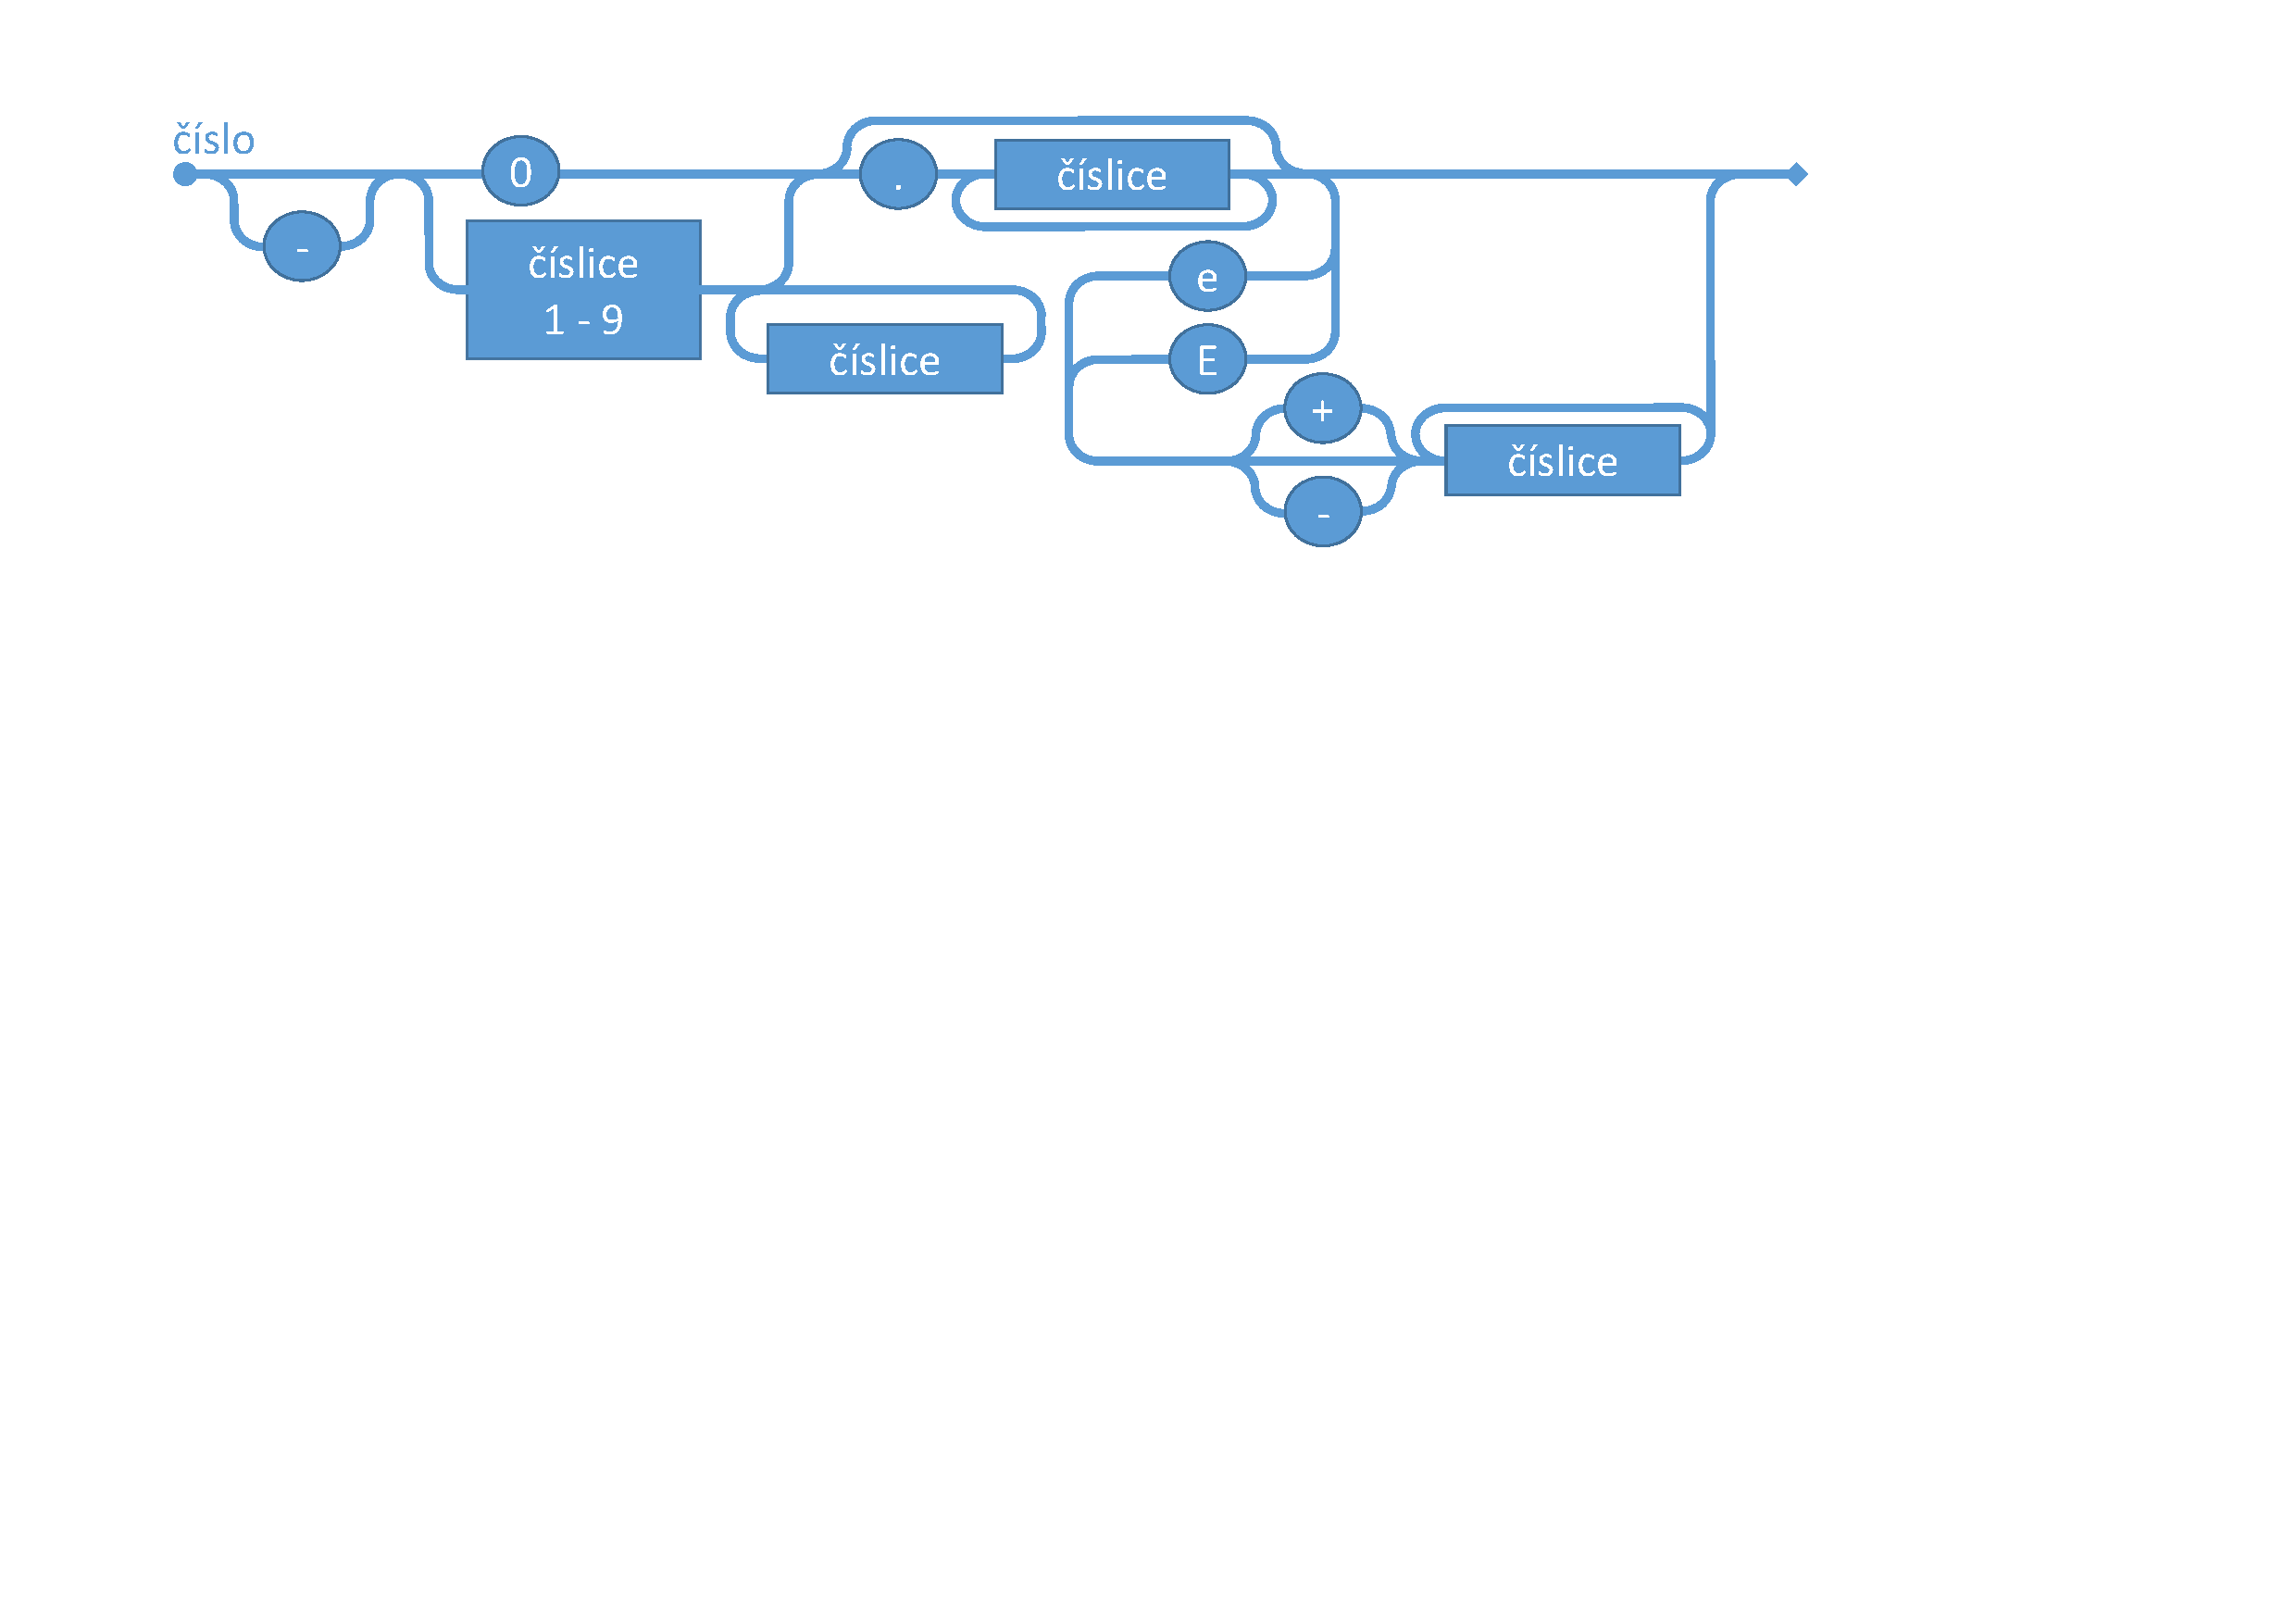
\includegraphics[trim=80 550 240 55, clip, angle=0, width=150mm]{cislo}
\caption{Struktura čísla}
\label{cislo}
\end{figure}

\subsubsection{Řetězce}
Řetězec je posloupnost Unicode znaků uvozená a zakončená znakem \texttt{\textquotedblright} (uvozovky). Mezi uvozovky mohou být zapsány všechny znaky kromě speciálních znaků, které jsou uvozeny tzv. únikovým znakem \texttt{\textbackslash} (zpětné lomítko), těmito znaky jsou například \texttt{\textquotedblright}, \texttt{\textbackslash}, \texttt{t} (znak tabulátoru), \texttt{n} (znak posunu kurzoru na nový řádek) a \texttt{r} (znak posunu kurzoru na začátek řádku, známý jako návrat vozíku) a další. Kompletní výčet je možné vidět na obrázku \ref{retezec} nebo v \cite{json}. Navíc je možné každý znak zapsat pomocí kombinace \texttt{\textbackslash u} a čtyřmístného hexadecimálního čísla odpovídajícího Unicode kódu požadovaného znaku. Řetězec obsahující pouze zpětné lomítko můžeme tedy zapsat následujícími způsoby: \texttt{\textquotedblright\textbackslash\textbackslash\textquotedblright}, \texttt{\textquotedblright\textbackslash u005c\textquotedblright} nebo \texttt{\textquotedblright\textbackslash u005C\textquotedblright} (u hexadecimálních čísel \texttt{A-F} nezáleží na velikosti).

\begin{figure}[!htb]
\centering
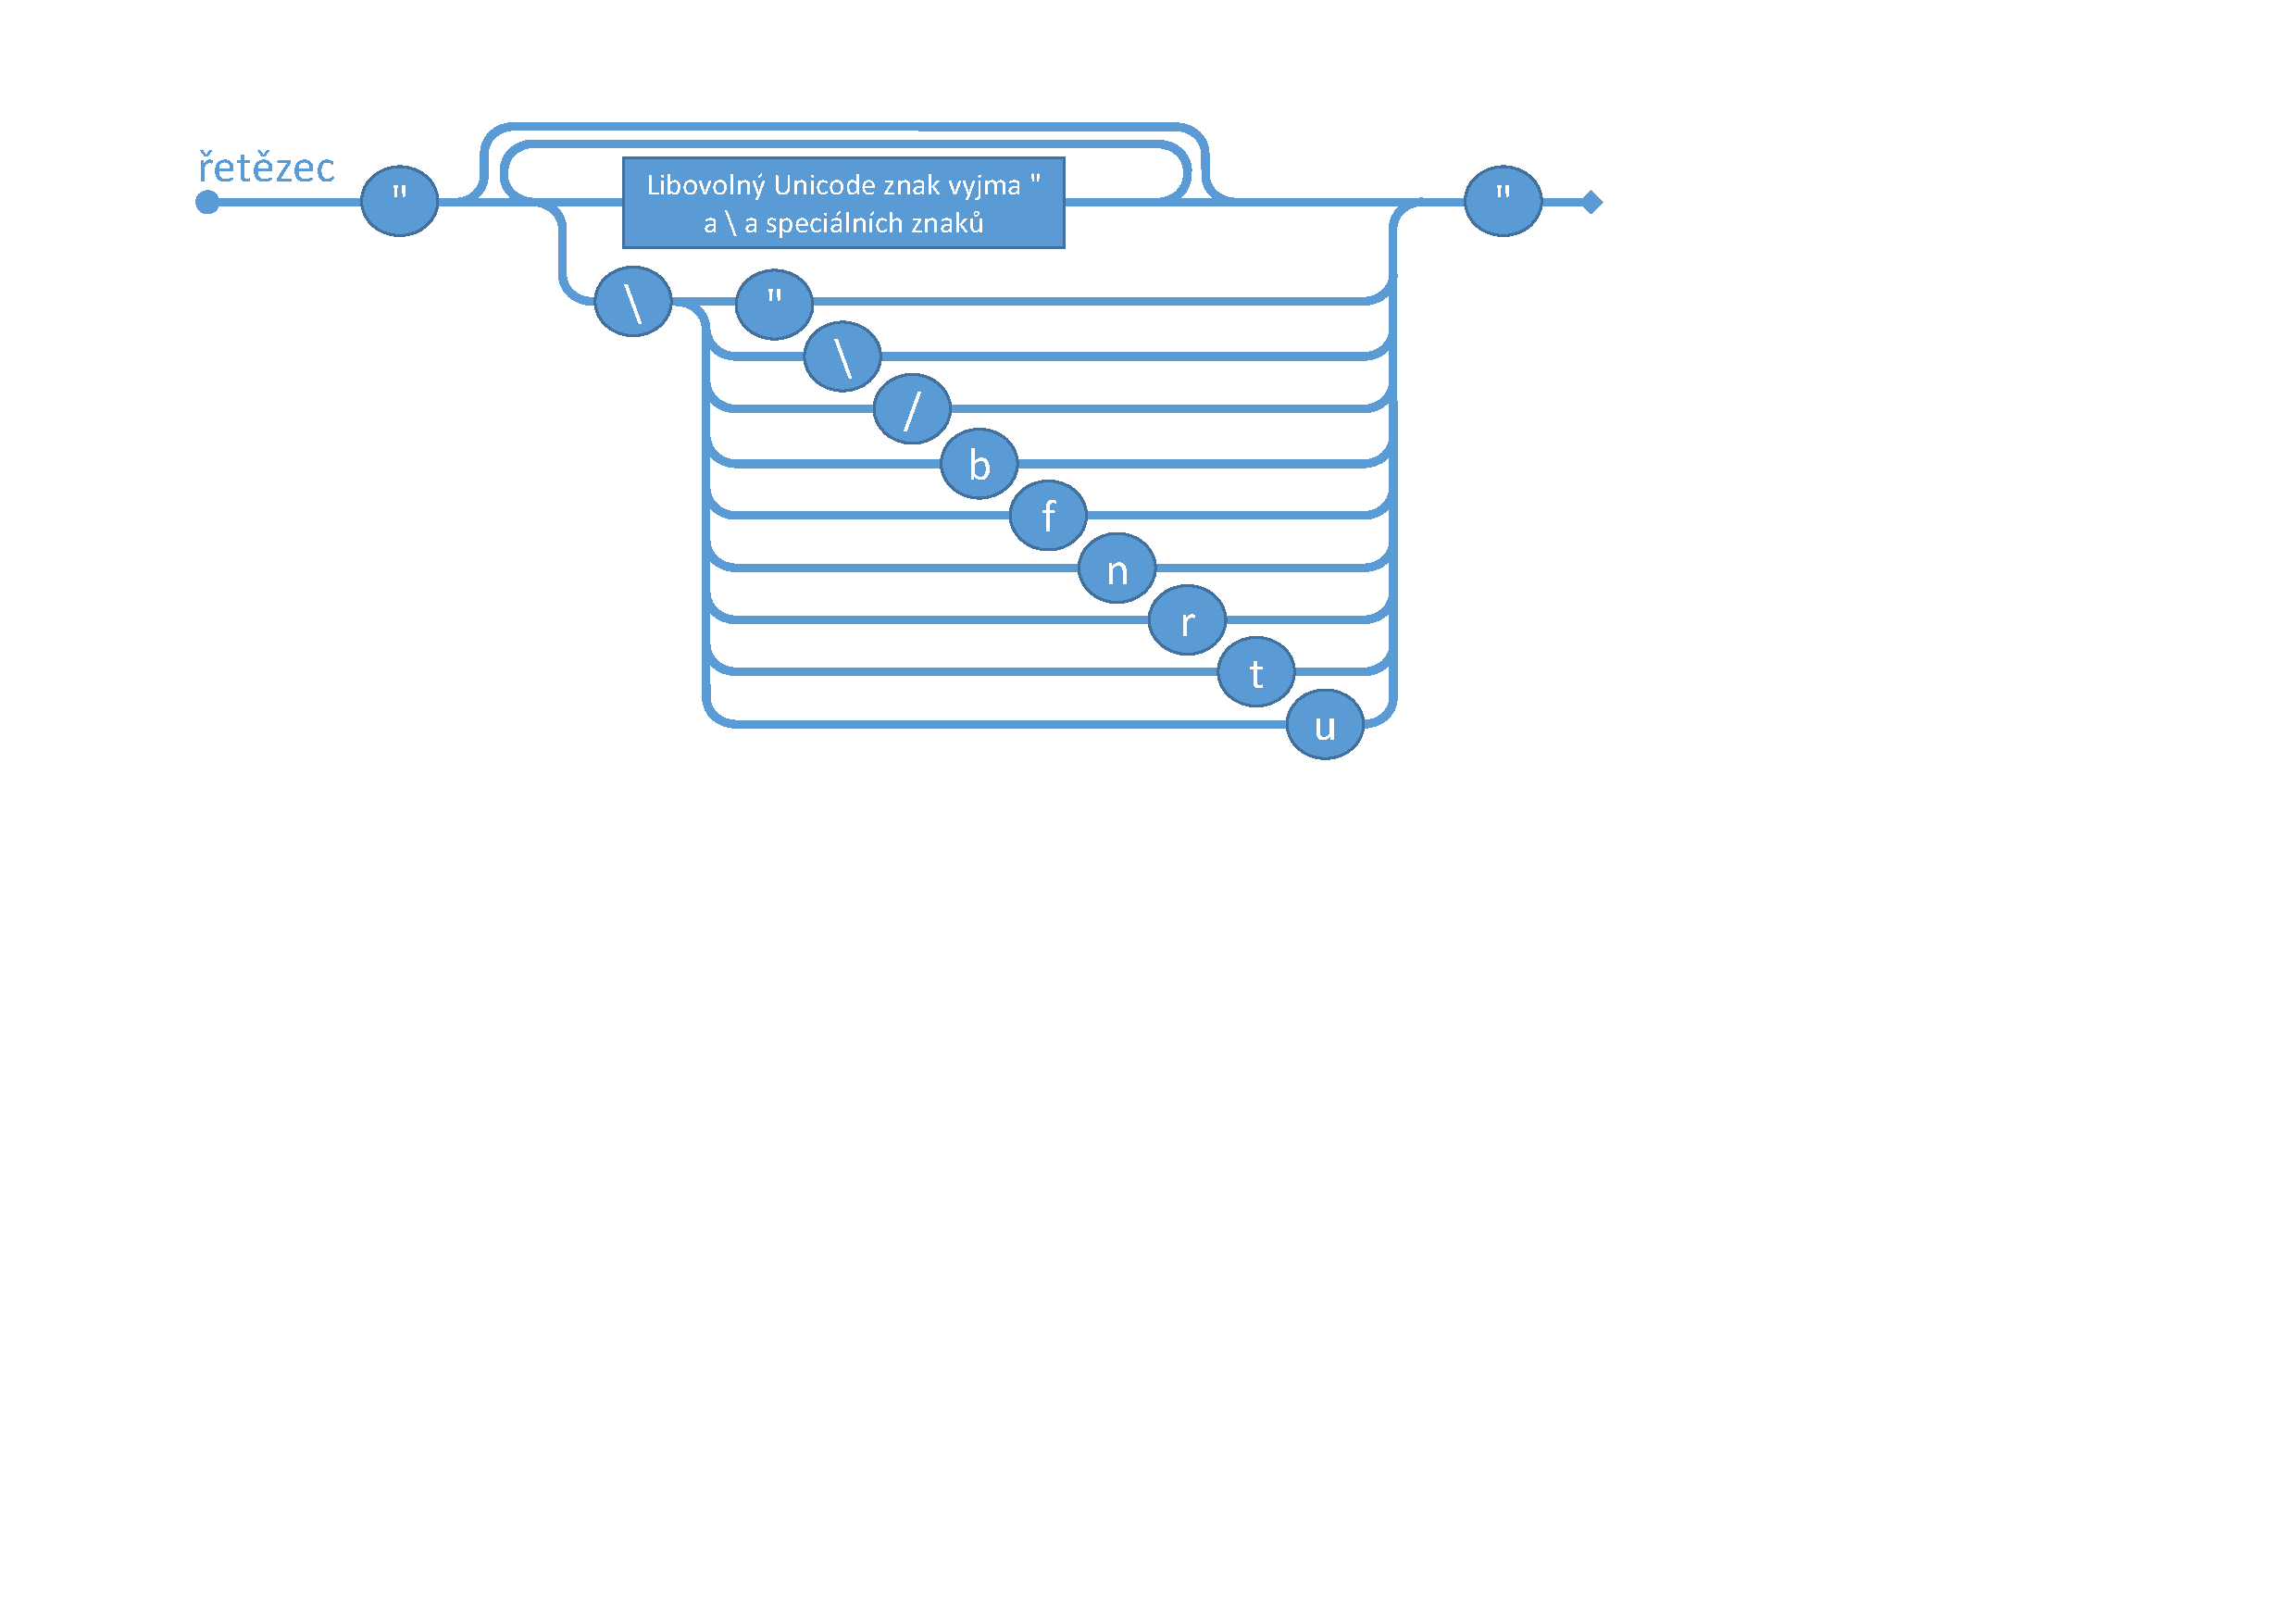
\includegraphics[trim=80 440 360 55, clip, angle=0, width=150mm]{retezec}
\caption{Struktura řetězce}
\label{retezec}
\end{figure}

\subsection{Vzorový příklad}
Stejně jako ve vzorovém příkladě \ref{xmlpriklad} ke XML, je zde popsána postavička Homera Simpsona včetně příbuzných, tentokrát ale v notaci JSON. Jde o objekt složený ze tří atributů, první dva mají hodnoty typu řetězec, k poslednímu \texttt{relatives} ale přísluší hodnota typu pole, ve kterém je vloženo pět příbuzných -- hodnot typu řetězec.

\texttt{\small\{\\
\hspace*{2mm}"firstName": "Homer",\\
\hspace*{2mm}"lastName": "Simpson",\\
\hspace*{2mm}"relatives": [\\
\hspace*{4mm}"Grandpa",\\
\hspace*{4mm}"Marge",\\
\hspace*{4mm}"Bart",\\
\hspace*{4mm}"Lisa",\\
\hspace*{4mm}"Maggie"\\
\hspace*{2mm}]\\
\} }

\subsection{Parsování}

\section{Vzájemné porovnání XML a JSON}

%Vybrat nějaké argumenty z diskusí a zapsat je tady pro porovnání

Na téma, zda je XML obecně lepší než JSON nebo naopak, bylo vedeno již nespočet diskusí. Argumentace obou stran diskuse je obvykle podložena jak teoretickou znalostí formátů, tak i praktickým použitím v reálných projektech. I přes to si myslím, že žádná diskuse nepřinesla jednoznačnou odpověď na výše položenou otázku, což samozřejmě pro některé konkrétní případy použití neplatí a volba jednoho z formátů je nutná nebo alespoň výhodnější. Ze svého zkoumání této problematiky si ale odnáším jeden podstatný závěr, který bych chtěl čtenáři zdůraznit: Vždy záleží na konkrétní situaci. Před samotným rozhodnutím, který z formátů využít, je vhodné zvážit důležité požadavky a do těchto úvah zahrnout klidně i další z existujících datových formátů.

Podíváme-li se znovu na vzorové příklady zápisu dat nebo položíme-li si vedle sebe stejná data zapsaná do obou formátů (viz příloha \ref{prilohaPorovnaniXmlJson}), můžeme lehce vidět vzájemnou podobnost. Ve své práci proto vycházím z předpokladu, že jsou oba formáty z hlediska toho, jaká data lze do nich zapsat, ekvivalentní. Respektive budu pro další porovnání používat pouze takový druh dat, který bude tento předpoklad splňovat.